\documentclass{beamer}
\usepackage{amsmath}
\usepackage{icomma}
\usepackage[utf8]{inputenc}
\usepackage[T1]{fontenc}
\usepackage{polski}
\usepackage[polish]{babel}
\usepackage{hyperref}
\usepackage{float}
\usetheme{Darmstadt}
\usecolortheme{rose}

% Naprawa nazw z angielskiego
\def\figureautorefname{Rysunek}

%Strona streszczenia
\newenvironment{abstractpage}
  {\cleardoublepage\vspace*{\fill}\thispagestyle{empty}}
  {\vfill\cleardoublepage}
  
%Samo streszczenie
\newenvironment{abstractsection}[1]
  {\bigskip\selectlanguage{#1}%
   \begin{center}\bfseries\abstractname\end{center}}
  {\par\bigskip}

%Ładne ułamki w jednostkach fizycznych
\sisetup{per-mode=symbol}%

\beamertemplatenavigationsymbolsempty
\setbeamertemplate{footline}[frame number]

\begin{document}
	\section{Wprowadzenie}
	\begin{frame}
		\title[Omnivelma]{Symulacja dookólnej bazy mobilnej}
		\author{Radosław Świątkiewicz}
		\date{\today}
		\institute{Wydział Elektroniki i Technik Informacyjnych \\ Politechnika Warszawska}
		\titlepage
	\end{frame}
	\begin{frame}
		\frametitle{Spis treści}
		\tableofcontents[currentsection]
	\end{frame}
	\begin{frame}
		\begin{description}
			\item[Autor] Radosław Świątkiewicz
			\item[Promotor] dr hab. inż. Wojciech Szynkiewicz \\ Zespół Programowania Robotów i Systemów Rozpoznających \\ Instytut Automatyki i Informatyki Stosowanej
		\end{description}
	\end{frame}
	
	\section{Cel}
	\begin{frame}
		\frametitle{Platforma dookólna}
		\begin{columns}[c]
			\column{0.5\textwidth}
			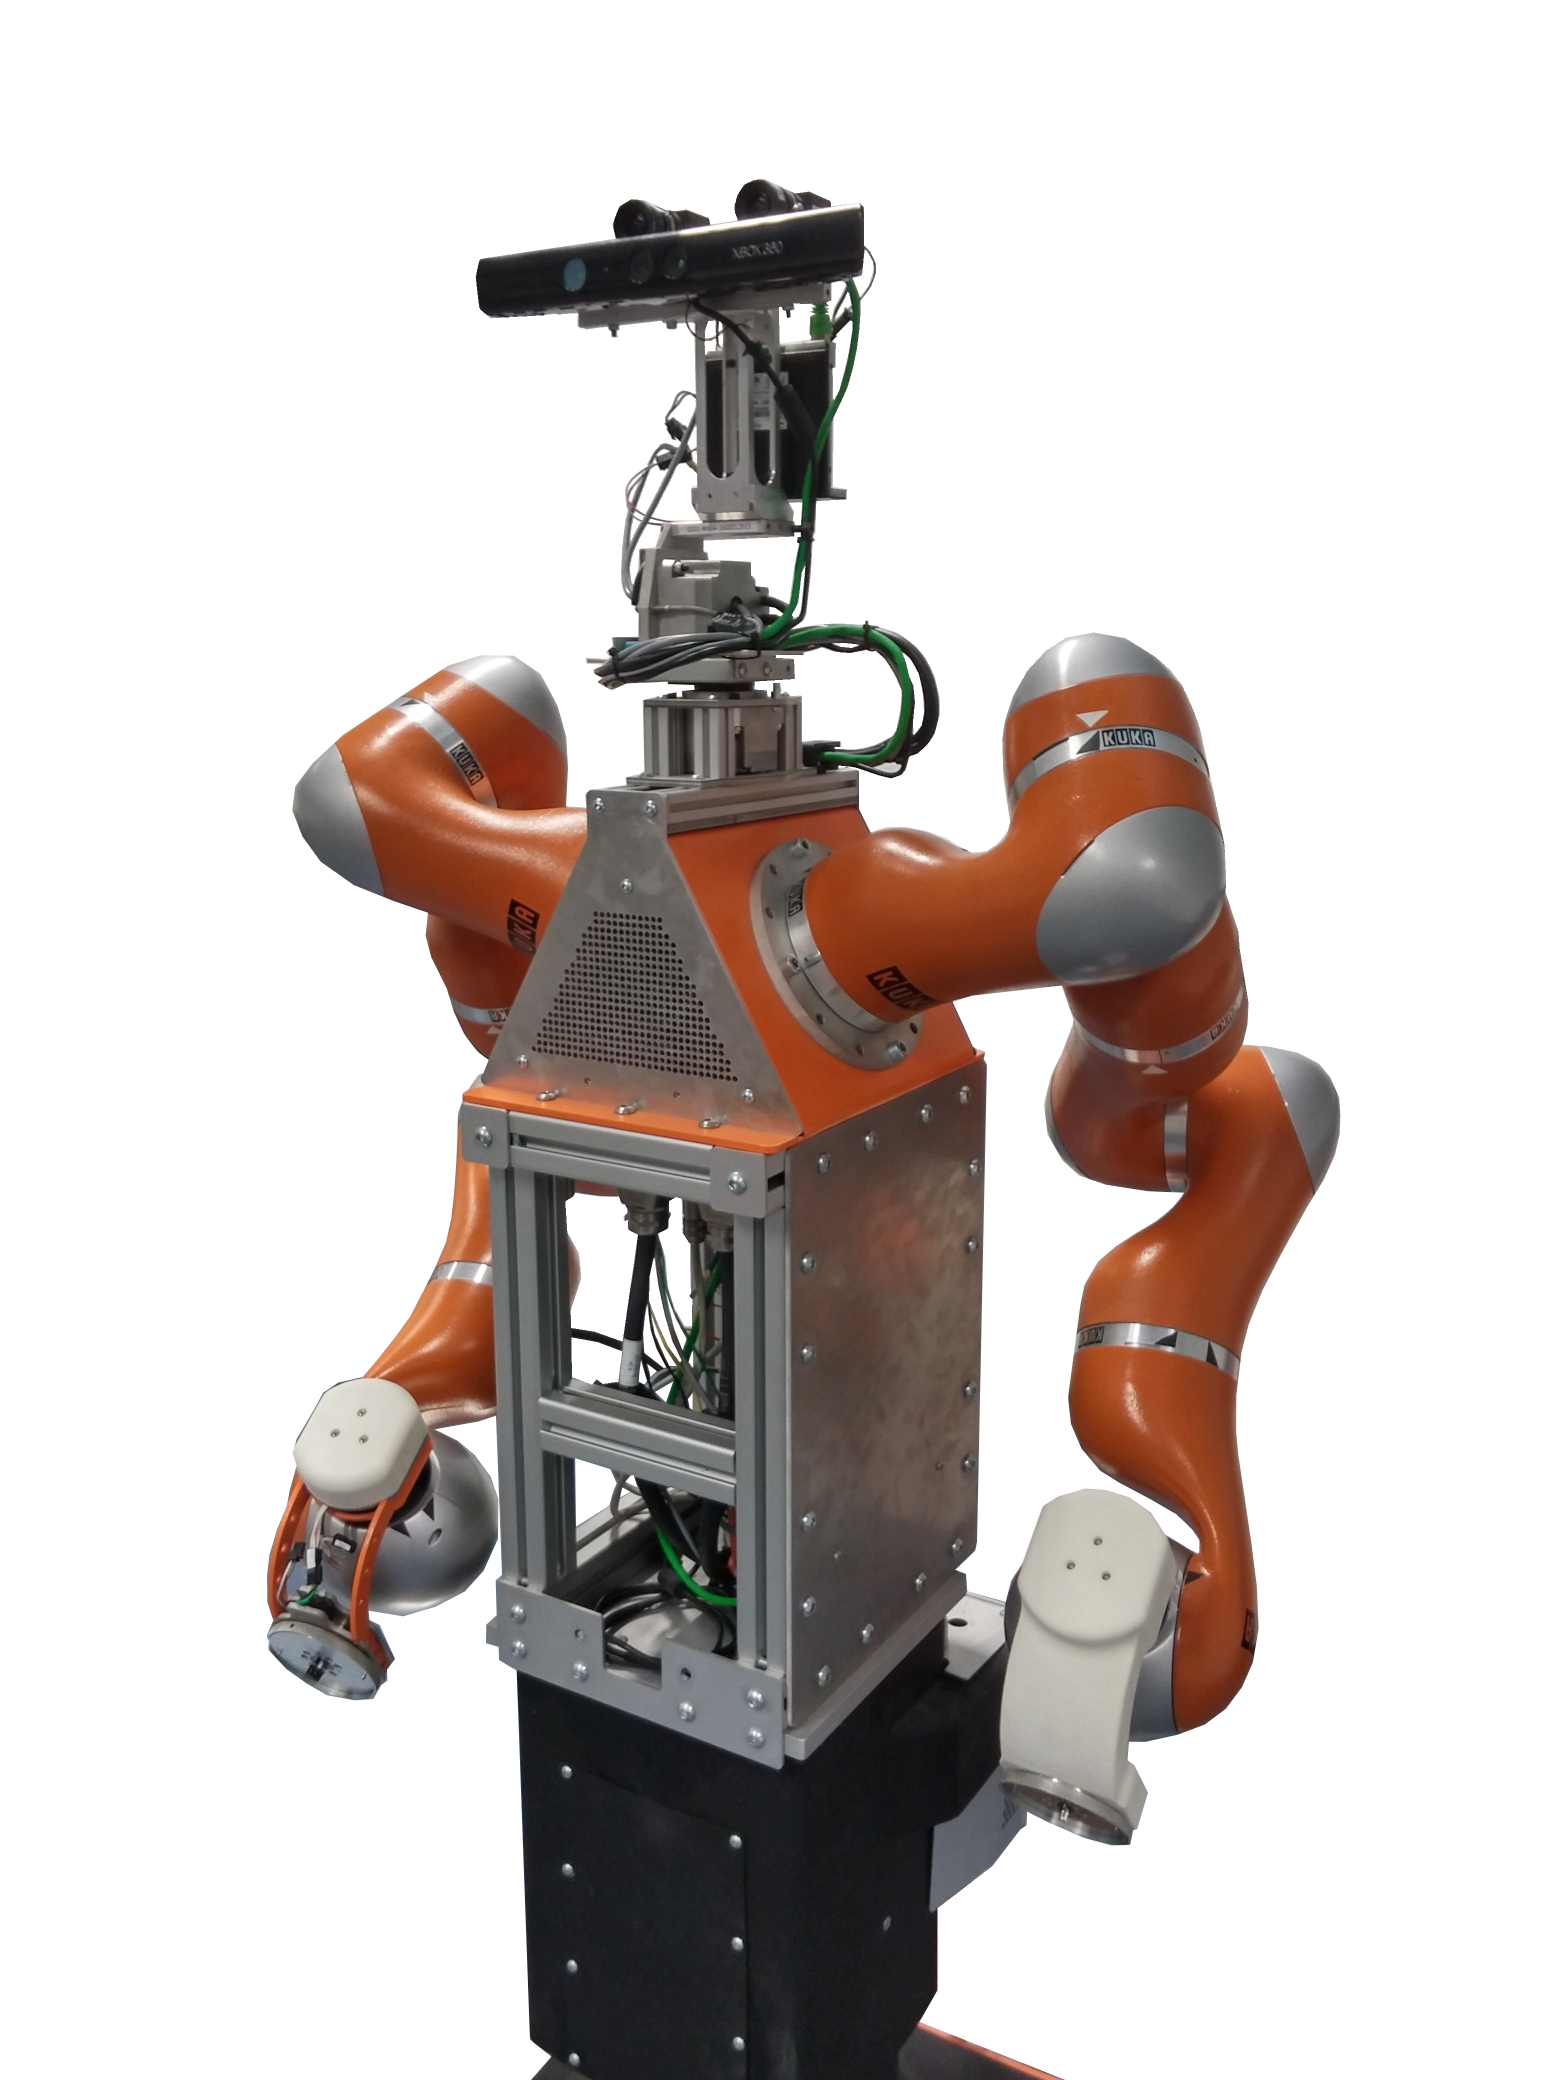
\includegraphics[width=0.8\textwidth]{graphics/velma.png} \\
			Robot manipulacyjny Velma
			\column{0.5\textwidth}
			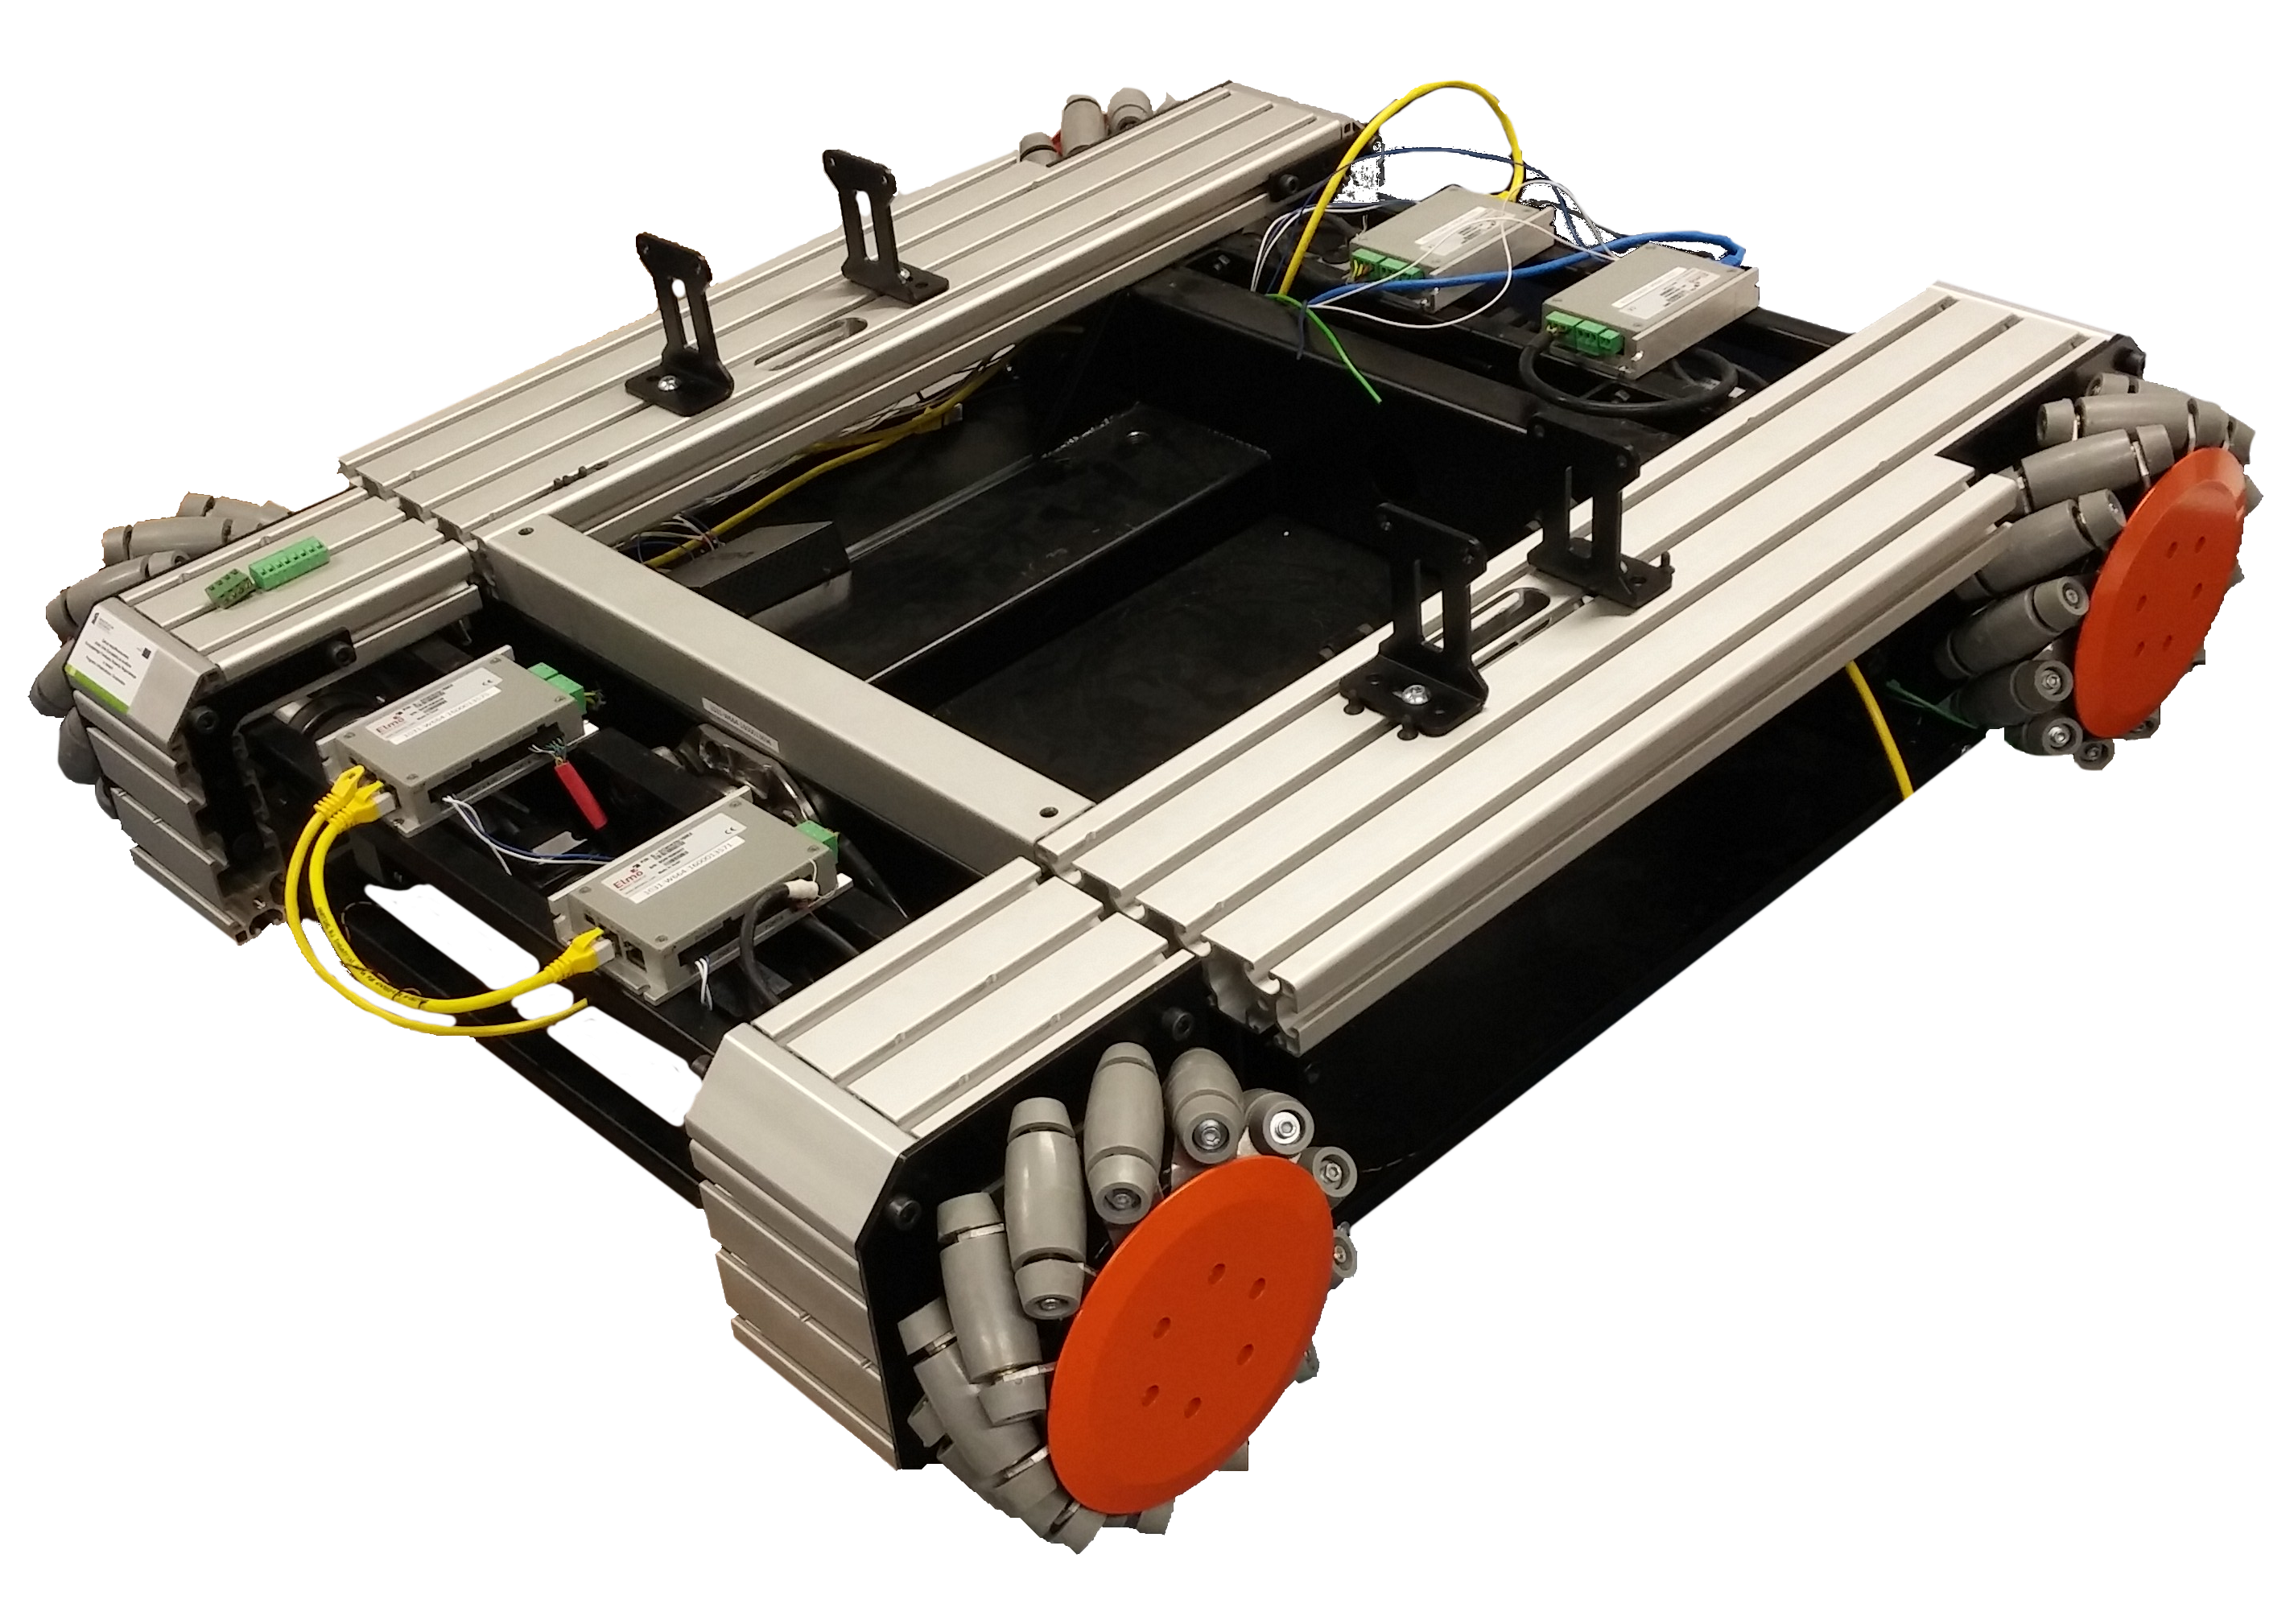
\includegraphics[width=\textwidth]{graphics/omnivelma.png} \\
			Platforma na kołach Mecanum
		\end{columns}
	\end{frame}
	\begin{frame}
		\frametitle{Co to jest model}
		Po co potrzebny jest model:
		\begin{itemize}
		 \item Pozwala bezpiecznie testować nowe oprogramowanie.
		 \item Przyspiesza budowanie algorytmów sterowania.
		 \item Ułatwia przeprowadzanie skomplikowanych testów.
		 \item Daje możliwość implementacji nieistniejących czujników.
		\end{itemize}
		Wymagania:
		\begin{itemize}
		 \item Reaguje na siły w podobny sposób, co robot.
		 \item Przyjmuje takie samo sterowanie.
		 \item Generuje odpowiednie dane z wirtualnych czujników.
		\end{itemize}
	\end{frame}
	
	\section{Platforma}
	\begin{frame}
		\frametitle{Koła Szwedzkie (Mecanum)}
		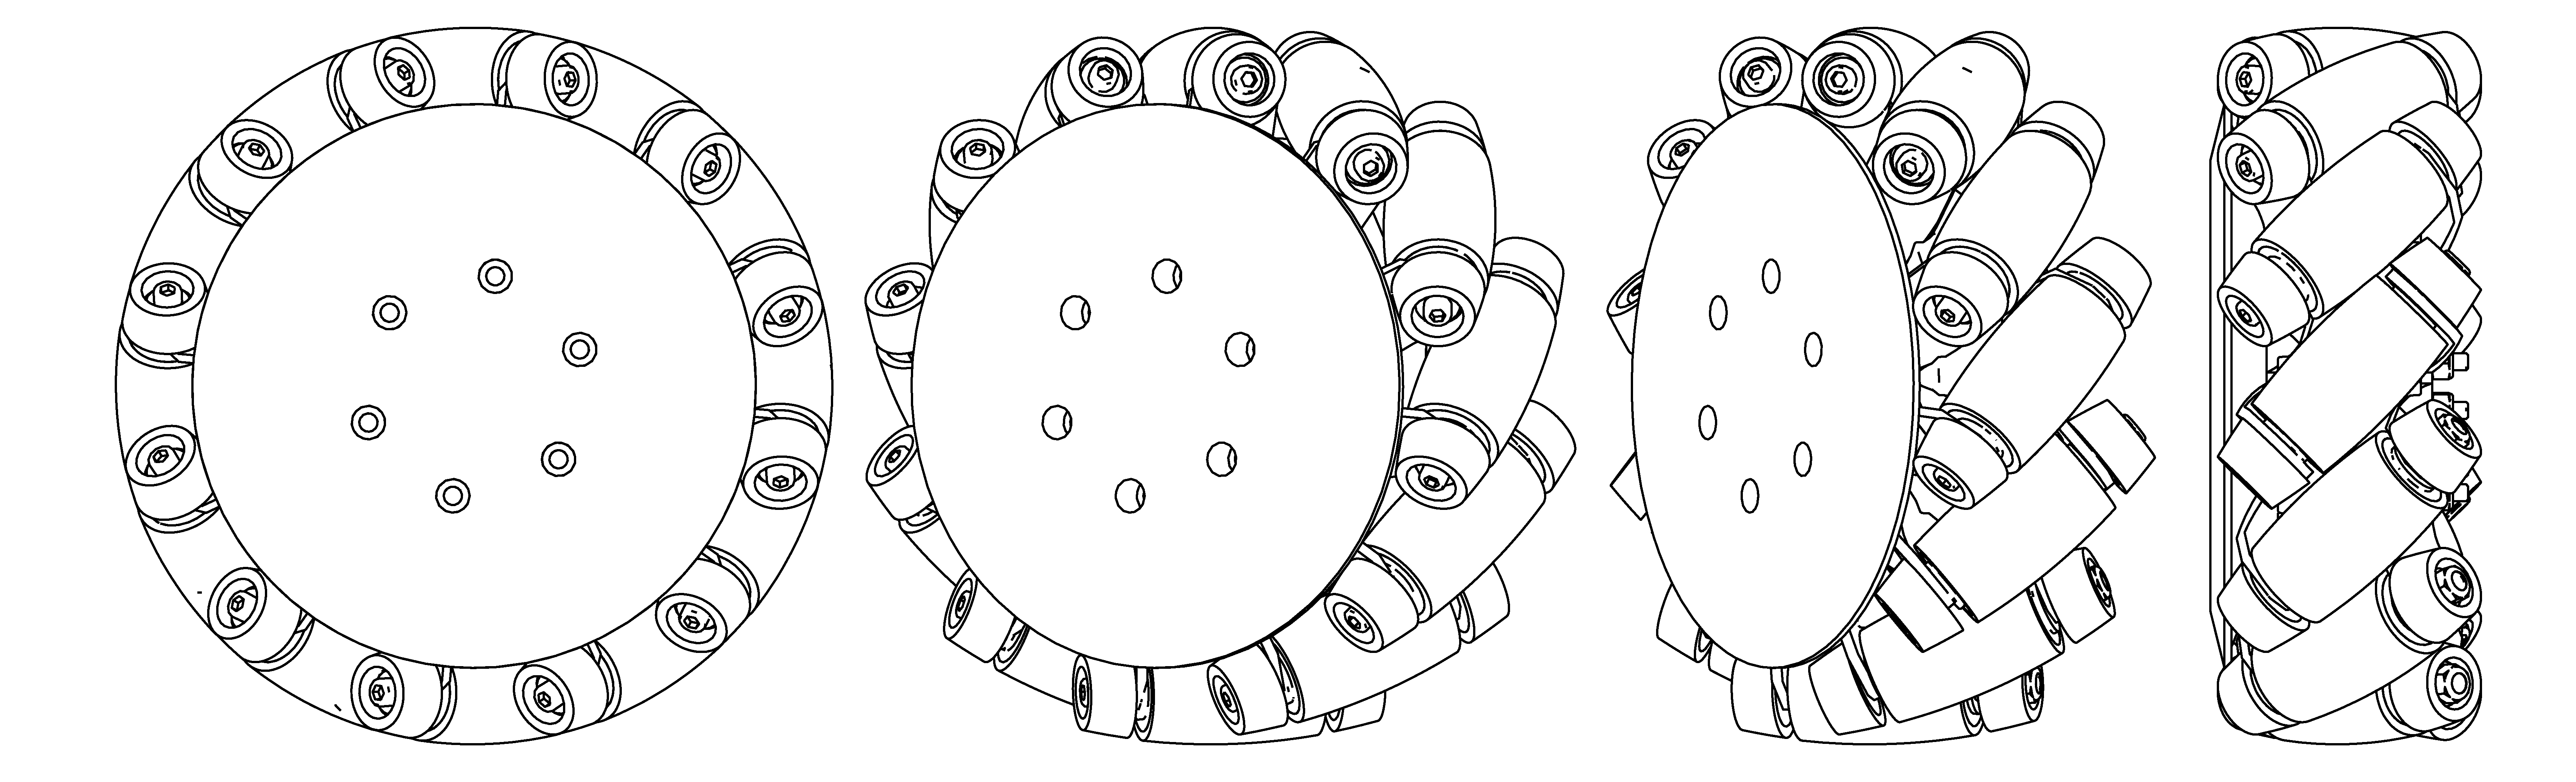
\includegraphics[width=\textwidth]{graphics/wheel.pdf}
	\end{frame}
	\begin{frame}
		\frametitle{Kierunki ruchu}
		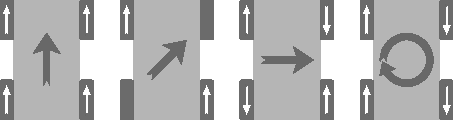
\includegraphics[width=\textwidth]{graphics/dirs.pdf}
	\end{frame}


	
	
	
\end{document}